% chapters/results.tex
\chapter{Results}
\label{ch:results}

% ---------- Chapter 5: Results ----------

\begin{table}
\centering

\begin{threeparttable}

\caption{
Best-fit parameters for single-parameter models to SNe Ia data.
The accuracy of the results is limited to $1\times10^{-3}$ due to
the grid spacing.
}
\label{tab:5.1}

\small

\begin{tabular}{@{}lccccc@{}}
\toprule

SNe Ia sample
&
$\Omega_M$
&
$w_0$
&
$w_1$
&
$\gamma$
&
$H_0$\tnote{c}
\\

\midrule

Constitution\tnote{a}
&
$0.29 \pm 0.02$
&
$-1.0 \pm 0.06$
&
$-0.26 \pm 0.4$
&
$0.06 \pm 0.1$
&
$64.95 \pm 0.2$
\\

Constitution 0.2x\tnote{a}
&
$0.29 \pm 0.01$
&
$-1.0 \pm 0.01$
&
$-0.24 \pm 0.07$
&
$0.07 \pm 0.03$
&
$65.01 \pm 0.03$
\\

Gold\tnote{a}
&
$0.34 \pm 0.04$
&
$-0.92 \pm 0.1$
&
$0.73 \pm 0.7$
&
$-0.33 \pm 0.3$
&
$63.55 \pm 0.3$
\\

Gold 0.2x\tnote{a}
&
$0.34 \pm 0.01$
&
$-0.92 \pm 0.02$
&
$0.73 \pm 0.1$
&
$-0.32 \pm 0.05$
&
$63.6 \pm 0.06$
\\

Union\tnote{a}
&
$0.29 \pm 0.03$
&
$-1.1 \pm 0.08$
&
$-0.24 \pm 0.5$
&
$0.04 \pm 0.2$
&
$69.68 \pm 0.3$
\\

Union 0.2x\tnote{a}
&
$0.29 \pm 0.01$
&
$-1.1 \pm 0.02$
&
$-0.24 \pm 0.08$
&
$0.03 \pm 0.03$
&
$69.76 \pm 0.04$
\\

SNAP\tnote{b}
&
$0.30 \pm 0.01$
&
$-1.0 \pm 0.02$
&
$0.01 \pm 0.1$
&
$0.0 \pm 0.04$
&
$72.05 \pm 0.1$
\\

SNAP 0.2x\tnote{b}
&
$0.30 \pm 0.01$
&
$-1.0 \pm 0.01$
&
$0.0 \pm 0.02$
&
$0.0 \pm 0.01$
&
$72.01 \pm 0.03$
\\

\bottomrule
\end{tabular}

\begin{tablenotes}
\footnotesize

\item[a]
Results obtained using the published supernova compilations.
The value of $H_0$ used in the original calibration is not known.

\item[b]
Results obtained using data sets generated with
$H_0 = 72\ \mathrm{km\,\mathrm{s}^{-1}\,\mathrm{Mpc}^{-1}}$.

\item[c]
Converted from the fitted quantity $h/h_{72}$ using
$H_0 = 100 \left( h/h_{72} \right) \times 72 \mathrm{km}\,\mathrm{s}^{-1}\,\mathrm{Mpc}^{-1}$.
The values of $h/h_{72}$ were recorded to an accuracy of $ 1 \times 10^{-3}$.

\end{tablenotes}

\end{threeparttable}

\end{table}


\begin{table}[htbp]
\centering

\begin{threeparttable}

\caption{
Comparison of best-fit values and 68\% confidence levels with values
quoted in the original SNe surveys. The accuracy of the results is
limited to $1\times10^{-3}$ due to the grid spacing.
}
\label{tab:5.2}

\begin{tabular}{@{}lccc@{}}

\toprule

\multirow{2}{*}{Compilation}
&
\multicolumn{3}{c}{Parameter value $\Omega_M$}
\\

\cmidrule(lr){2-4}

&
Survey
&
Own results
&
Reduced-error set
\\

\midrule

Constitution &
$0.281^{+0.037}_{-0.016}$ &
$0.291 \pm 0.02$ &
$0.290 \pm 0.01$
\\

Gold\tnote{a} &
$0.28 \pm 0.04$ &
$0.342 \pm 0.04$ &
$0.342 \pm 0.01$
\\

Union &
$0.287^{+0.029}_{-0.027}\,\text{(stat)}
^{+0.039}_{-0.036}\,\text{(sys)}$ &
$0.285 \pm 0.03$ &
$0.287 \pm 0.01$
\\

\midrule

\multirow{2}{*}{Compilation}
&
\multicolumn{3}{c}{Parameter value $w_0$}
\\

\cmidrule(lr){2-4}

&
Survey
&
Own results
&
Reduced-error set
\\

\midrule

Constitution &
$-0.913^{+0.066}_{-0.068}\,\text{(stat)}
\pm 0.11\,\text{(sys)}$ &
$-1.03 \pm 0.06$ &
$-1.03 \pm 0.01$
\\

Gold &
$-0.8^{+0.6}_{-1.0}$ &
$-0.934 \pm 0.1$ &
$-0.928 \pm 0.02$
\\

Union &
$-0.969^{+0.059}_{-0.063}\,\text{(stat)}
^{+0.063}_{-0.066}\,\text{(sys)}$ &
$-1.07 \pm 0.08$ &
$-1.06 \pm 0.02$
\\

\bottomrule

\end{tabular}

\begin{tablenotes}
\footnotesize
\item[a] Gold set assumes a priori $\Omega_M = 0.28 \pm 0.04$.
\end{tablenotes}

\end{threeparttable}

\end{table}


\begin{table}[htbp]
\centering

\begin{threeparttable}

\caption{One-parameter deviations from the $\Lambda$CDM values from the results in
\cref{sec:5.1}. ``Gold'' is the best-fit values from the Gold sample;
``Const./Union'' is the average of the best-fit values from the two data sets;
``Compromise'' is the average of all three and ``WMAP+BAO+Const.'' represent the
most up-to-date estimates from CMB, BAO and the Constitution set, copied from
\cite{Komatsu2010}. Uncertainties quoted are 68\% CL for Gold and WMAP+BAO+Const.
and the standard error of the 68\% CL for the other two columns.}
\label{tab:5.3}

\begin{tabular}{@{}lcccc@{}}
\toprule
Parameter & Gold\tnote{a} & Const./Union & Compromise & WMAP+BAO+Const. \\
\midrule

$\Omega_M$ &
$0.34 \pm 0.04$ &
$0.29 \pm 0.03$ &
$0.31 \pm 0.02$ &
$0.282^{+0.015}_{-0.016}$ \\

$w_0$ &
$-0.92 \pm 0.1$ &
$-1.1 \pm 0.07$ &
$-1.0 \pm 0.06$ &
$-0.980 \pm 0.053$ \\

$w_1$ &
$0.73 \pm 0.7$ &
$-0.25 \pm 0.45$ &
$0.08 \pm 0.39$ &
$0.38^{+0.66}_{-0.65}$ \\

$\gamma$ &
$-0.33 \pm 0.3$ &
$0.05 \pm 0.16$ &
$-0.08 \pm 0.15$ &
$0$ by definition \\

\bottomrule
\end{tabular}

\begin{tablenotes}
\footnotesize
\item[a] Sign of $w_0$ corrected from a misprint in the original source.
\end{tablenotes}

\end{threeparttable}

\end{table}


The project produces four different outputs for each data set: the Markov chains used to produce the posterior PDFs, the posteriors themselves, credible regions for the $\binom{4}{1}$ parameters and $\binom{4}{2}$ pairs thereof and the distance modulus curves for those parameter values which have the greatest likelihood. Of these, the latter two are useful for analysis. It is also desirable to compare the results from this project to those obtained by the supernova search teams themselves and by alternative methods of parameter estimation, namely anisotropies in the cosmic microwave background and baryon acoustic oscillations in elliptical galaxies. For one of the models to be a viable alternative we require that the best-fit values from all of the observational data sets agree, i.e. they all lie within the others’ 68\% credible regions. This is due to the lack of tension between the three Ia SNe sets asserted by \cite{Kwan2009}: if the data from all observations are consistent, then those parameters which have a high probability of producing one set’s distance moduli must also have a high probability of producing the others. Conversely, if the credible regions from the three observational sets do not overlap in a certain subspace, then we may discard the subset of models which span that subspace. This is a qualitative measure which may be quantitatively expressed by calculating the Bayes factors from the posteriors, using a technique described in the further work (\cref{sec:6.1}). 

Firstly we examine the credible regions from the single-parameter models in \cref{sec:5.1}. (For brevity I omit similar analysis for the individual parameters in two-parameter models.) I then examine the possibility of correla- tions between parameters shown in the two-parameter models in \cref{sec:5.2}. In \cref{sec:5.3} I add \bao{} results from the Sloan Digital Sky Survey and \cmb{} results from the seven-year Wilkinson Microwave Anisotropy Probe to the 2d credible regions in order to obtain tighter constraints on the cosmological parameters. Lastly in \cref{sec:5.4} I examine the astrophysical and cosmological implications of a non-$\Lambda$CDM universe.

\section{Parameter values from 1-dimensional models}
\label{sec:5.1}

\begin{figure}
\centering
\staticfigure[.8\textwidth]{figures/chapter5/fig5.1a-f.png}{Posterior PDFs for each parameter in the single-parameter models (not marginalised over $H_0$). Each data set is denoted by a different colour, with the $1\sigma$ credible region in the lightest shade and $3\sigma$ the darkest. Regions in black are outside $3\sigma$. Larger versions of the $1\sigma$ credible regions are contained in \cref{app:large-figures}. (b) shows the Hubble parameter $h/h_{72}$, (c) the matter density $\Omega_m$ ; (d) the constant equation of state parameter $w_0$; (e) the varying equation of state parameter $w_1$; and, (f) the mixing factor $\gamma$.}
\end{figure}

The single-parameter models represent the simplest modification to the concordance $\Lambda$CDM model, containing only matter (both baryonic and dark) and a cosmological constant. Each posterior represents the probability that a value from the continuum set by the prior is the value which created the data. Thus, the mode is the value with the highest likelihood of being the value in the observable universe. The error is taken to be the width of the 68\% credible region by convention. The results are summarised in \cref{tab:5.1}. Plotting the credible regions themselves (\cref{fig:fig5.1a-f}) allows a comparison of the 1$\sigma$, 2$\sigma$, 3$\sigma$ errors for each data set.
   
The first step is to determine the value of $H_0$ used by the different SNe observing groups. This serves two purposes: it acts as a plausibility check on the smaller-error data (since these sets should agree (i.e. their 1$\sigma$ intervals should overlap) with the $H_0$ value of the sets on which they are based) and it justifies the use of the Hubble parameter as a free parameter for all models. If the $H_0$ value were the same for all data sets, I would have been able to set it as a constant, thus reducing the dimensionality of the model parameter spaces and shortening the length of the Markov chains. We find in \cref{fig:fig5.1a-f}(b) and \cref{tab:5.1} that only between the Gold and Constitution sets is there overlap in the 3$\sigma$ regions and that the credible regions of each reduced-error set are entirely enclosed by the same regions in the corresponding original set. Therefore we can conclude that a different value for the Hubble constant was applied to each normal-error set and that the reduced-error sets are behaving plausibly. It is vital to stress that I have not discovered a value for the Hubble constant: these values were applied arbitrarily by the different SNe search teams and then marginalised over as a nuisance parameter. This is in contrast to the other credible regions, which do suggest a value for their parameters.

The single-parameter models indicate that only minor modifications to the concordance model produce a better fit to the observed data. All three posteriors from the observational data give parameter values with consistent agreement, i.e. the 1$\sigma$ confidence regions overlap. 

The cosmological matter density $\Omega_m$ (\cref{fig:fig5.1a-f}(c)) has a best-fit value of $0.29$ across the Constitution and Union sets and their reduced-error sets and this agreement is confirmed by the overlap of the $1\sigma$ regions. The Gold set $1\sigma$ region intersects the $1\sigma$ regions of the Constitution and Union sets at $\Omega_m = 0.31$, however one must look at the 2$\sigma$ confidence regions before an agreed value is found between these and the Gold 0.2x set. The Gold and Gold 0.2x sets have a best-fit parameter value of $\Omega_m$ = 0.34, which is ruled out at 3$\sigma$ for the Constitution and Union sets and 4$\sigma$ for the corresponding 0.2x error sets. This demonstrates that the smaller-error sets amplify the calibration differences between the Gold set and the later Constitution and Union sets.

Similarly, the constant parameter $w_0$ (\cref{fig:fig5.1a-f}(c)) in the dark energy equation of state is well-agreed upon by all three observational data sets, which display overlap in their $1\sigma$ credible regions at $w_0 = -1$, although one must go to $2\sigma$ for overlap between the $1\sigma$ Gold 0.2x region and either the Constitution or Union sets. Once again the Gold 0.2x set does not overlap with the other two reduced-error sets. The agreement between the Constitution and Union samples is not as clear as for the matter density, as their best-fit values no longer agree, nor is there overlap at $1\sigma$ between their reduced-error sets. Nevertheless, the considerable overlap between the normal-error sets suggests that a cosmological constant $w_0 = -1$ can produce the observed SNe data.
   
There is no clear value for a time-varying dark energy equation of state which would better explain the distance moduli from the SNe data. This is once again due to the lack of consistency between the Gold set and the Union and Constitution sets. The latter two sets and their reduced-error sets all have a best-fit value around $w_1 = -0.25$ \cref{tab:5.1} whereas the Gold and Gold 0.2x sets share a best-fit value of $w_1 = 0.73$. The Gold best-fit value is ruled out at $3\sigma$ by the other two sets, whose best-fit value is slightly more plausible, lying in the 2$\sigma$ region for the Gold set. The 1$\sigma$ regions for all three observed sets intersect at $w_1 = 0.2$ in \cref{fig:fig5.1a-f}(e) whereas the concordance value of $w_1 = 0$ is in the 2$\sigma$ region for the Gold set. This suggests the inclusion of a small, positive variation in the equation of state. Given the difference in best-fit values between the Gold set and either the Constitution and Union sets, any modification would need to be tested against a sample of SNe at higher redshift (when the time-varying parameter has greater effect) to ascertain which of $w_1 \sim -0.25$, $w_1 \sim 0.2$ or $w_1 \sim 0.73$ is the most suitable value.
   
The interaction parameter $\gamma$ in \cref{fig:fig5.1a-f}(f) presents the same dilemma: although there is overlap of the 1$\sigma$ credible regions for the Gold and Union sets (the Constitution and Gold sets intersect at their 1 - 2$\sigma$ boundaries), the best-fit values lie in the 2$\sigma$ region of the other set. The considerable overlap between the Constitution and Union sets and their respective reduced-error sets is again present, all of which prefer (Table 5.1) a small positive interaction parameter to none at all. In contrast the Gold and Gold 0.2x sets prefer a negative interaction parameter approximately one order of magnitude greater than the Union and Constitution sets’ best-fit value. Thus the observational data propose a contradicting energy transfer: $\gamma > 0$ represent the transfer of energy from dark energy into matter, whereas $\gamma < 0$ represents the opposite. There is no clear value which satisfies all observational sets.

The projected sets from the \snap{} survey were artificially generated, so they do not propose parameter values for the observable Universe. As with the $H_0$ credible regions, we are interested solely in the reproduction of the values used to generate the distance moduli and the width of the region compared to the other data sets. From \cref{tab:5.1} we see that both the normal and reduced-error sets display the same best-fit values: moreover, these correspond to the concordance model values which were used to generate the data. This demonstrates that the Markov chains were run for a sufficient time to achieve convergence with the true posterior (i.e. stable equilibrium). Although the Snap 0.2x set display 1$\sigma$ regions which are far narrower than the other data sets, the Snap errors are of the same order of magnitude as those of the reduced-error sets. This suggests that a recalibration of existing data which reduces fivefold the uncertainty in distance moduli may produce equally tight constraints on the cosmological parameters as the pessimistic view of results from a new survey.

Comparison to the original papers in \cref{tab:5.2} is reassuring: the posteriors do not contradict the existing results for the Union and Constitution sets. Unfortunately, the tension in single-parameter models between the Gold set and these two sets is not reproduced in the original papers. This is because their value for the matter density was fixed at $\Omega_m = 0.28 \pm 0.04$, rather than the 0.3 which I used, so their constraints on the dark energy equation of state cannot be readily compared (\cite{Riess2007}). Their decision to use $\Omega_m$ as a Gaussian prior with maximum at 0.28 and width 0.04 came from large-scale structure measurements to obtain $\Omega_m$ h and Cepheids (another type of standard candle) to find a value for $H_0$ \cite{Riess2007}, so the validity of their results are sensitive to changes in the accepted values for $H_0$ . Therefore it is difficult to obtain a meaningful comparison between my single-parameter results and those of Riess et al. The 0.2x sets produce narrower confidence intervals due to the scaling of the error bars and the same best-fit values because they share the same data points as the observed data. Although this situation is less than ideal because the errors which contribute to the $\mu(z)$ uncertainties also produce scatter in the data points, there was no information available to guide any ”correction” to this scatter, so alterations would have generated meaningless data. The reproduction of best-fit values acts as a ”sanity check” to confirm convergence of the Markov chains. Quantitative attempts to compare how the parameter uncertainties scale with those in the distance moduli are limited by the resolution of the binning. Nevertheless, for both the normal- and reduced-error sets, my best-fit results do fit within and the 1$\sigma$ limits do overlap with (where comparison is appropriate) the 1$\sigma$ limits quoted in the papers.


\section{Degeneracies between parameters from 2-dimensional models}
\label{sec:5.2}

\begin{figure}
\centering

\staticsubfigure{figures/chapter5/fig5.2a.png}{Constitution}
\hfill
\staticsubfigure{figures/chapter5/fig5.2b.png}{Union}

\medskip

\staticsubfigure{figures/chapter5/fig5.2c.png}{Gold}
\hfill
\staticsubfigure{figures/chapter5/fig5.2d.png}{SNAP}

\caption{Credible regions illustrating correlations between the matter density and constant equation of state parameter for the different data sets: (a) Constitution; (b) Union; (c) Gold; and (d) SNAP.}
\label{fig:fig5.2}
\end{figure}

\begin{figure}
\centering

\staticsubfigure{figures/chapter5/fig5.3a.png}{Constitution}
\hfill
\staticsubfigure{figures/chapter5/fig5.3b.png}{Union}

\medskip

\staticsubfigure{figures/chapter5/fig5.3c.png}{Gold}
\hfill
\staticsubfigure{figures/chapter5/fig5.3d.png}{SNAP}

\caption{Credible regions illustrating correlations between the matter density and varying equation of state parameter for the different data sets: (a) Constitution; (b) Union; (c) Gold; and (d) SNAP.}
\label{fig:fig5.3}
\end{figure}

\begin{figure}
\centering

\staticsubfigure{figures/chapter5/fig5.4a.png}{Constitution}
\hfill
\staticsubfigure{figures/chapter5/fig5.4b.png}{Union}

\medskip

\staticsubfigure{figures/chapter5/fig5.4c.png}{Gold}
\hfill
\staticsubfigure{figures/chapter5/fig5.4d.png}{SNAP}

\caption{Credible regions illustrating correlations between the matter density and interaction parameter for the different data sets: (a) Constitution; (b) Union; (c) Gold; and (d) SNAP.}
\label{fig:fig5.4}
\end{figure}

\begin{figure}
\centering

\staticsubfigure{figures/chapter5/fig5.5a.png}{Constitution}
\hfill
\staticsubfigure{figures/chapter5/fig5.5b.png}{Union}

\medskip

\staticsubfigure{figures/chapter5/fig5.5c.png}{Gold}
\hfill
\staticsubfigure{figures/chapter5/fig5.5d.png}{SNAP}

\caption{Credible regions illustrating correlations between the constant and varying equation of state parameters for the different data sets: (a) Constitution; (b) Union; (c) Gold; and (d) SNAP. The black line marks the ``CMB wall'' $w_0 + w_1 = 0$.}
\label{fig:fig5.5}
\end{figure}

\begin{figure}
\centering

\staticsubfigure{figures/chapter5/fig5.6a.png}{Constitution}
\hfill
\staticsubfigure{figures/chapter5/fig5.6b.png}{Union}

\medskip

\staticsubfigure{figures/chapter5/fig5.6c.png}{Gold}
\hfill
\staticsubfigure{figures/chapter5/fig5.6d.png}{SNAP}

\caption{Credible regions illustrating correlations between the constant equation of state and interaction parameters for the different data sets: (a) Constitution; (b) Union; (c) Gold; and (d) SNAP.}
\label{fig:fig5.6}
\end{figure}

\begin{figure}
\centering

\staticsubfigure{figures/chapter5/fig5.7a.png}{Constitution}
\hfill
\staticsubfigure{figures/chapter5/fig5.7b.png}{Union}

\medskip

\staticsubfigure{figures/chapter5/fig5.7c.png}{Gold}
\hfill
\staticsubfigure{figures/chapter5/fig5.7d.png}{SNAP}

\caption{Credible regions illustrating correlations between the varying equation of state and interaction parameters for the different data sets: (a) Constitution; (b) Union; (c) Gold; and (d) SNAP.}
\label{fig:fig5.7}
\end{figure}

\begin{figure}
\centering
\begin{minipage}[c]{0.48\textwidth}
  \centering
  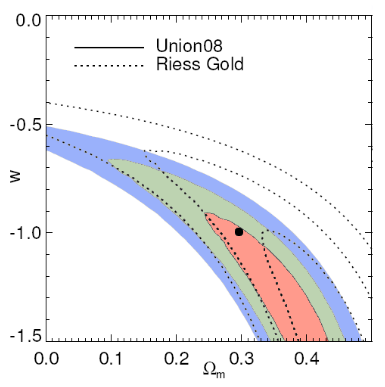
\includegraphics[width=\linewidth]{figures/chapter5/fig5.8.png}
\end{minipage}
\hfill
\begin{minipage}[c]{0.48\textwidth}
  \caption{Comparison of the $(\Omega_M , w_0)$ credible regions from the Union and Gold (Riess) data modified from \cite{Kowalski2008}. I have coloured the image for better contrast: red, green and blue filled contours show $1, 2, 3\sigma$ regions from the Union set and the empty contours the Gold set. I also added a dot to show the position of the $\Lambda$CDM model. Image credit: Fig. 13 from \cite{Kowalski2008}.}
  \label{fig:fig5.8}
\end{minipage}
\end{figure}

\begin{figure}
\centering
\begin{minipage}[c]{0.48\textwidth}
  \centering
  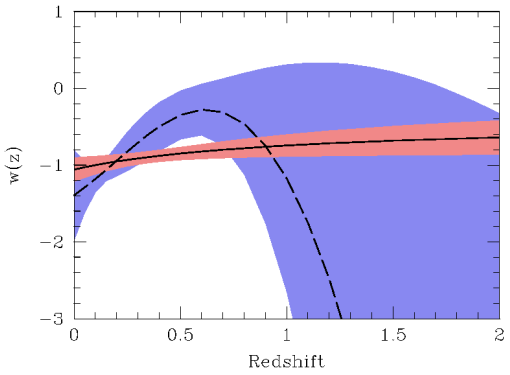
\includegraphics[width=\linewidth]{figures/chapter5/fig5.9.png}
\end{minipage}
\hfill
\begin{minipage}[c]{0.48\textwidth}
  \caption{$90\%$ confidence limits on $w(z)$ for the linear parameterisation $w(z) = w_0 + w_1 \frac{z}{1+z}$ (red) and a quartic polynomial $\sum_{i=0}^{4} w_i (\ln{}(1 + z))^{i} $ (blue) using the Gold set. The best-fit equations of state are the black lines: solid for the linear parameterisation and dashed for the polynomial.  Image credit: Fig. 10 in \cite{Riess2007}.}
  \label{fig:fig5.9}
\end{minipage}
\end{figure}


The two-dimensional models illustrate degeneracies between the different parameters. This causes difficulty if one wishes to estimate the cosmological parameters from Ia SNe alone: the data is sufficient to constrain the parameters pairwise, but insufficient to determine a value for them separately. Linear degeneracy clearly exists for the pairs $(\Omega_m , \gamma)$ (\cref{fig:fig5.4}), $(w_0 , w_1 )$ (\cref{fig:fig5.5}), whereas the other four combinations $(\Omega_m , w_0)$ (\cref{fig:fig5.2}), $(\Omega_m , w_1 )$ (\cref{fig:fig5.3}), $(w_0 , \gamma)$ (\cref{fig:fig5.6}), $(w_1 , \gamma)$ (\cref{fig:fig5.7}) display degeneracies which have a more complex curved shapes. These shapes are linear for intermediate values of the parameters, however they curve to become horizontal or vertical at either end of the credible regions.  In these locations the parameters are completely non-degenerate: a precise value for one parameter contributes no information about the value of the other. Despite this, the reduced-error and Snap sets suggest linear degeneracy may emerge from these credible regions if the distance modulus uncertainties are reduced.

The $(\Omega_m , w_0)$ credible regions replicate the results from the SNe search teams for the three observational sets. In particular \cite{Kowalski2008} confirms the discrepancy (\cref{fig:fig5.8}) I found between the Gold (\cref{fig:fig5.2}c) and Union (\cref{fig:fig5.2}b) samples. 
The $\Lambda$CDM model falls in the 1$\sigma$ region for both Constitution (\cref{fig:fig5.2}a) and Union sets, whereas it is more unlikely to be predicted from the Gold data, as it lies in the 2$\sigma$ region. The smaller-error sets have 3$\sigma$ regions which rule out the $\Lambda$CDM values and are entirely enclosed by the 1$\sigma$ regions from the respective observational sets, with the ratio of areas within 1$\sigma$ indicating a better-than-linear scaling relationship between uncertainties in $\mu(z)$ and uncertainties in the values of the cosmological parameters. The dots at the position of the $\Lambda$CDM parameter values show that only the Constitution set favour the concordance model, whereas the Union set places it at the $1-2\sigma$ boundary and the Gold set firmly in the 2$\sigma$ credible region. 
In comparison to the Constitution set, the Union set favours more negative values of the constant equation of state parameter $w_0$ for equivalent values of the fractional matter density $\Omega_m$ whereas the Gold set favours more negative $w_0$ and larger values of $\Omega_m$ . There is overlap between the 1$\sigma$ credible regions for the observational sets, however this region does not include the concordance model.

Including a time-varying equation of state 
\begin{equation*}
w(z) = \Lambda + w_1 \frac{z}{1+z} = -1 + w_1 \frac{z}{1+z}    
\end{equation*}
produces the credible regions for $(\Omega_m , w_1)$, which do not favour the $\Lambda$CDM model. 
The Constitution data (\cref{fig:fig5.4}a) places the $\Lambda$CDM parameter values at the $1 - 2\sigma$ boundary, the Gold data in the 2$\sigma$ region and the Union data at the $2-3\sigma$ region boundary, while the reduced-error sets all place $(\Omega_m , w_1) = (0.3, 0)$ outside 3$\sigma$. 
At first glance, this strongly suggests that a negative time variation in $w(z)$ is far more likely than a constant. However, this result may simply be a consequence of fixing $w_0$ at a value which does not produce a good fit to the data,\footnote{This is seen by the intersection of $w_0 = -1$ (and $w_1 = 0$ because it is fixed) with the $(\Omega_m , w_0)$ credible regions, discussed in the previous paragraph.} which causes the $w_1$ value to decrease in an attempt to improve the fit. This is supported by the degeneracy between the two parameters in the dark energy equation of state shown in the $(w_0 , w_1)$ credible regions. A model varying the fractional matter density and both equation of state parameters is necessary to gain more insight into this problem.

Next we examine the linear $(w_0 , w_1)$ correlation (Fig. ??). One may question whether this is a consequence of the equation of state constraints or truly a product of the available data. Although a flat prior was assumed for all of the parameter values, the form of the dark energy equation of state 
\begin{equation*}
    w(z) = w_0 + w_1 \frac{z}{1+z} 
\end{equation*}
acts as a strong prior, placing (perhaps unjustifiably) strong constraints on the behaviour of $w(z)$. \cref{fig:fig5.9} demonstrates this by plotting the 95\% credible region (2$\sigma$ confidence $z$ limits) on $w(z)$ for the linear parameterisation 
\begin{equation*}
    w(z) = w_0 + w_1 \frac{z}{1+z} 
\end{equation*}
(red) and a quartic polynomial 
\begin{equation*}
    w(z) = \sum_{i=0}^{4} w_i \left[ \ln(1+z) \right]^i
\end{equation*}
(blue) using the Gold set \cite{Riess2007}. The behaviour of the best-fit models for the dark energy equation of state 
differs dramatically: the linear parameterisation is (by definition) monotonically increasing as $z \rightarrow{} \infty{}$, however the quartic admits a non-monotonic evolution with recent changes (at $z < 0.1$) in $w(z)$. This suggests that the linear parameterisation generates artificially well-constrained results for w(z). Conversely, one may argue that the use of the more general equation of state is unwarranted (it merely expresses our gross ignorance, rather than being physically well-motivated,so the results may depend strongly upon the choice of prior \cite{Efstathiou2008}), as the Gold set does not have sufficient SNe (only 23 at $z > 1$) \cite{Riess2007} to place limits on such a general w(z). This problem may be resolved by using the $> 1000$ samples expected from observations with survey telescopes such as SNAP/WFIRST, the Large Synoptic Survey Telescope\footnote{LSST \url{http://www.lsst.org}} and the Panoramic Survey Telescope and Rapid Response System\footnote{Pan-STARRS \url{http://pan-starrs.ifa.hawaii.edu/public}} \cite{Leibundgut2008}. These projects will provide large, homogeneous data sets with increased numbers of SNe at z > 1, which will give tighter constraints on $w(z)$ at (relatively) high redshift \cite{Leibundgut2008}.

Finally we analyse the credible regions including interaction, for which there are no existing results from the SNe survey teams. The ($\Omega_m$ , $\gamma$) models show a linear correlation between the fractional matter density and the interaction parameter. Both the Constitution (\cref{fig:fig5.4}a) and Union (\cref{fig:fig5.4}b) sets suggest that the concordance model is plausible, since ($\Omega_m$ , $\gamma$) = (0.3, 0) lies within the 1$\sigma$ regions, however the Gold data once again disagrees, placing it only within 2$\sigma$. The Constitution 0.2x set also favours the $\Lambda$CDM model, however the Gold 0.2x and Union 0.2x sets neither agree well with $\Lambda$CDM nor their normal-error counterparts (the 1$\sigma$ regions intersect the 2 and 3$\sigma$ region of the normal-error sets). 
This is probably caused by a convergence problem with the Markov chains: both of these data–model combinations had to be run for unusually large step sizes before the resulting histogram was smooth, but they may have needed even longer before the histogram converged to the posterior. Highly negative values of $\gamma$ represent transfer of energy from matter into dark energy, resulting in $\Omega_m \rightarrow{} 0$ as $z \rightarrow{} -1$. As this result is not indicated by the observational data, these two results remain a curiosity. Overall, $\gamma$ = 0 lies within the 1$\sigma$ regions for values of $\Omega_m$ which are observationally likely, (0.25 . $\Omega_m$ . 0.5), so at this stage no interaction remains a probable result. 
The credible regions for ($w_0$ , $\gamma$) (\cref{fig:fig5.6}) and ($w_1$ , $\gamma$) (\cref{fig:fig5.7}) have degeneracies which are unlikely to be resolved. This is because the interaction in the adiabatic Friedmann equation \cref{eq:1.10} can be represented as an effective non-constant equation of state [3, 67], which contributes an additional term to w(z). As $\gamma \rightarrow{} -1$ it loses its degeneracy with $w_1$ : the credible regions (\cref{fig:fig5.7}) become horizontal, so a particular value for $\gamma$ places no constraint upon the value for $w_1$ . At the limit:

\begin{subequations}
\label{eq:5.1}
\begin{align}
    \frac{\dd{\Omega}_{m}}{\dd{z}} &=
    \frac{1}{1+z} \left(
        3 \Omega_{m} + \frac{1}{H(z)}
    \right)
    \label{eq:5.1a} \\
    \frac{\dd{\Omega}_{X}}{\dd{z}} &=
    \frac{1}{1+z} \left(
        3 \Omega_{X} \left(
            1 + w_{0} + w_{1} \frac{z}{1+z}
        \right)
        - \frac{1}{H(z)}
    \right)
    \label{eq:5.1b}
\end{align}
\end{subequations}

so in the past, as $z \rightarrow{} \infty{}$, the effect of $H(z)$ will swamp the effect of any values of $w(z)$ and the value of $\Omega_X$ will be negative,\cite{vanOsten2006} which is physically impossible (as it is a fractional density). The credible regions \cref{fig:fig5.2,fig:fig5.3,fig:fig5.4,fig:fig5.5,fig:fig5.6,fig:fig5.7} show that a large section of the 2d parameter space often lies within the 1$\sigma$ credible region, illustrating that the Friedmann equations may produce exceedingly similar distance modulus curves for very different initial conditions (fits to the data are given in §B). Therefore one must look for other observational data which does not display the same degeneracy\footnote{This statement is true only for $\Lambda$CDM-based models with a dark energy equation of state based on a barotropic model. More exotic possibilities such as the ”doomsday” and braneworld models do not display opposing degeneracies: see \cite{Rubin2008} for a summary of SN+\cmb{}+\bao{} credible regions with more exotic models.} in order to obtain tight constraints (on the order of those for the one-parameter models). 
Fortunately, the two other sources used for cosmological parameter estimation are complementary to SNe: both the \cmb{} and \bao{} display the opposite degeneracy (see \cref{sec:5.3}), at least for $\Omega_m$ , $w_0$ and $w_1$. It remains to be seen whether similar relationships exist for $\gamma$.







\section{Improving constraints: combination with CMB and BAO data}
\label{sec:5.3}

\begin{figure}
\centering
    \staticfigure{figures/chapter5/fig5.10.png}{$68.3\%$, $95.4\%$ and $99.7\%$ confidence level contours on $w_1$ (here $w_a$) and $w_0$ for a flat Universe. The Union SN set was combined with CMB or BAO constraints (left) and the SN+CMB+BAO constraints with and without the SNe systematics removed (right). The diagonal line represents $w_0 + w_a = 0$: the likelihoods based on observational data remain below it, favouring matter domination at $z \gg 1$.  Image credit: Fig. 16 in \cite{Kowalski2008}.}
\end{figure}

\begin{figure}
\centering
    \staticfigure{figures/chapter5/fig5.11.png}{Comparison of $(\Omega_M , w_0)$ credible regions from the Constitution data when two different light curve fitters are used to find the luminosity of the SNe. Left: SALT; right: MCLS2k2. Notice the shift in the position of the $\Lambda$CDM parameter values (the dot) with no change in the SNe observed, merely the data calibration. Image credit: Fig. 4 from \cite{Hicken2009}.}
\end{figure}


Tightening of cosmological parameter constraints can be achieved by combining SNe data with a range of other methods for estimating the parameters, foremost amongst which are multipoles in the power spectra from the cosmological microwave background (\cmb{}) \cite{LewisBridle2002,Spergel2007,Komatsu2010,Dunkley2009} and the correlation func- tion for luminous red galaxies from baryon acoustic oscillation (\bao{}) measurements \cite{Eisenstein2005,Carroll2001,Percival2007}. These measurements are sometimes referred to as ”standard rulers” because they directly measure fundamental cosmological distances \footnote{The ”standard candle” measures the luminosity distance because the luminosity of the object is independent of its local environment, so the ratio of the (corresponding) distance between two standard candles depends only on the intervening spatial curvature (given by the FLRW metric). Similarly, the ”standard ruler” measures the angular diameter distance because the ratios of angle subtended on the sky depends only on the spatial curvature via the FLRW metric. \cite{Hobson2006}}. 

A full estimate of the cosmological parameters from such sources requires a similar process\footnote{A summary of the \bao{} process is provided in \cite{vanOsten2006}§2.; for the \cmb{} an example of parameter extraction is \cite{LewisBridle2002} while the parameters extracted from this are summarised in \cite{vanOsten2006,Carroll2001}.} to this project: generating the relevant observational data from different values of the cosmological parameters and using a Markov chain Monte Carlo algorithm to move through the parameter space based on an acceptance/rejection scheme (e.g. Metropolis-Hastings, although much effort has been put into generating efficient schemes purely for the \cmb{} analysis \cite{Christensen2001,Dunkley2005,LewisBridle2002} ). Although credible regions for the parameters $(\Omega_m , w_0 , w_1 )$ are available from the \cmb{} \cite{Spergel2007,Komatsu2010,Dunkley2009} and $(\Omega_m , w_0)$ from \bao{} measurements \cite{Eisenstein2005,Percival2007}, they are not in a form which enabled me to compare them directly to my own results (except by sight).

A trend throughout the results has been tension between the parameter estimation produced by the Gold set and that produced by the Union and Constitution sets, which is emphasised by the lack of overlap in the credible regions for the Gold 0.2x set and the Constitution/Union 0.2x sets. This lack is easily explained if one considers the formation of the projected SNAP sets. The (unknown) parameter values for our Universe would produce a $\mu(z)$ curve according to the Friedmann equations \cref{eq:1.4}, the luminosity distance formula \cref{eq:1.15} and the theoretical distance modululs formula \cref{eq:1.13}. The $\mu(z)$ points from observations of Type Ia SNe must be calculated from the pragmatic distance modulus formula \cref{eq:1.14} once their luminosities (hence luminosity distances) are found from a light-curve fitter: the choice of corrections to obtain \cref{eq:1.13} from \cref{eq:1.14} and the choice of light curve fitter to determine \cref{eq:1.15} create a particular scatter of the data points around the \lq\lq{}true\rq\rq{} $\mu(z)$ curve. Uncertainties in these choices and limitations on the instrument precision and calibration create error bars about the data points. In this way, the jiggled Snap and Snap 0.2x sets were generated from a known set of cosmological values. The 0.2x sets for Constitution, Gold and Union have reduction in the error bars, but not in the scattering (for reasons detailed in \cref{sec:5.1}). Therefore the reduced error bars shrink the subset of parameter values which provide good fits to the data, while the same data points maintain the different scatters from the different data sets. This exaggerates the difference between the data sets, so overlap becomes more unlikely as the errors shrink. The difference between the data sets results mostly from the light curve fitters used to determine the SN luminosity: the Gold set uses the MLCS2k2 fitter \cite{Riess2007}, whereas the Union set uses the SALT fitter \cite{Kowalski2008}. The Constitution set was calibrated with four different fitters (SALT being the preferred fitter): their comparison of the effects of SALT and MLCS2k2 on the parameter estimates (\cref{fig:fig5.1a-f}) shows the same trend as my results, with the MLCS2k2 fitter placing the $\Lambda$CDM parameter values within 2$\sigma$ compared to 1$\sigma$ for SALT. The shift in credible regions increases when the SNe compared are different as well as the light-curve fitters. This illustrates the vital importance of developing new light-curve fitters which cause the credible regions from different fitters to converge. Until this task is completed, there will be uncertainties in the values of the cosmological parameters derived from SNe (see §C for more detail on this). The physical values of the parameters are obscured by our lack of knowledge of both the physical mechanisms associated with Type Ia SNe and the effect of the intervening environment \cite{Leibundgut2009}.


\section{Implications}
\label{sec:5.4}

Finding well-constrained estimates for the cosmological parameters is only one vital part of cosmology. Once the parameter values are established, one faces the task of developing physical theories which explain the parameter values. 

A particularly active field for cosmologists, quantum field theorists and particle physicists is the development of new models for dark energy, which can then be tested against the observational constraints \cite{LinderScherrer2009,Copeland2006}. The parameter values determine the density and expansion of the universe at the time of early structure formation \cite{Rees1998,Riess2009}, which will aid in developing models for the earliest astronomical objects, e.g. supermassive black holes and quasars (which may be the same thing) \cite{Rees1998}. 

In turn. this will shed light on early galaxy formation and may help solve the continuing problem of finding high-redshift objects with an age which is apparently greater than that of the Universe \cite{Krauss1997,Dunlop1996}.  Of particular concern is the need for astronomical studies to ensure that the criteria they use to judge formation models (e.g. globular cluster formation) are not cosmological-model-dependant. For example, the age of the Universe depends on the cosmological parameters (see the discussion in \cref{sec:2.4}), so this cannot be used to limit the age of early-forming objects such as globular clusters. Conversely, tight constraints on the age of the Universe (13.7 ± 0.2 Gyr for the $\Lambda$CDM model \cite{Barnes2005}) would provide an upper bound on the age of old, high-redshift objects (e.g. quasars \cite{Hasinger2002}, globular clusters \cite{Reid1998}, luminous elliptical galaxies \cite{Dunlop1996}), which would then act as a criterion for eliminating certain formation models for these objects which predicted an age older than the Universe \cite{Dunlop1996}. Beyond astronomy, the equation of state for dark energy will limit the possible physical methods by which the dark energy is generated. This impacts upon high energy physics theories which apply when the Universe is extremely young, such as supersymmetry and supergravity: see \cite{Copeland2006} for a review of this topic, which is beyond the scope of this project. Moreover, the cosmological parameter values predict the proportion of primordial light elements (H, D, He and Li) synthesized after the big bang \cite{Riess2009}, which acts as a test for dark energy represented by primordial quintessence fields \cite{Copeland2006}. The implications of a non-$\Lambda$CDM universe are present in diverse fields beyond cosmology.

In conclusion, there are currently three plausible groups of models which offer one-parameter deviations from the $\Lambda$CDM model: one favouring the Gold estimates, one favouring the Constitution/Union estimates and a compromise version that is a reasonable fit (within 1$\sigma$) for all three. The multiple- parameter models (of which only two-parameter models were examined here) have too many degeneracies to easily discern a best-fit value with 68\% confidence limits for each of the parameters. This problem may be resolved by combining the credible regions from Ia SNe with those from other data and redshift-distance relations to estimate the cosmological parameters, notably the angular diameter distance and data from the \cmb{} or \bao{}. Until the light-curve fitters which are used to reduce Type Ia SNe to standard candles are improved, the parameter estimates from different data sets (or even the same data but using different light curves) will give different credible regions for the parameters. Until then it is difficult to determine which of the families of parameter values \cref{tab:5.3} is closest to the true values for the observable Universe. Consequently, I conclude that the $\Lambda$CDM model is a reasonable approximation to the correct values which is currently unchallenged by parameter estimates derived from Type Ia SNe.